\documentclass[oneside,a4paper,12pt]{article}

\usepackage[]{hyperref}
\usepackage{tikz}
\usetikzlibrary{arrows,shapes,snakes,automata,backgrounds,petri,decorations.pathmorphing}
\usepackage[utf8]{inputenc}
\usepackage{tabularx}
\usepackage{textcomp}
\usepackage{lmodern}
\usepackage{listings}
\usepackage{amsmath}
\usepackage{float}
\usepackage{hyperref}
\usepackage{natbib}
\newcolumntype{M}[1]{>{\centering\arraybackslash}m{#1}}
\usepackage[nottoc,notlot,notlof,numbib]{tocbibind}
\usepackage[titletoc]{appendix}
\usepackage{titletoc}
\renewcommand{\appendixname}{Annexure}
\renewcommand{\bibname}{References}
\setcounter{secnumdepth}{5}

\usepackage{float}
\usepackage{subcaption}
\usepackage{multirow}

\usepackage[ruled,vlined]{algorithm2e}

\begin{document}

\setlength{\parindent}{0mm}
\begin{center}

\includegraphics[width=100pt]{assets/iitb_logo.png} \\
\vspace{20pt}
{\bfseries INDIAN INSTITUTE OF TECHNOLOGY BOMBAY \\}
 \vspace*{2\baselineskip}
{\bfseries Project Report on \\}
 \vspace*{1\baselineskip}
{\bfseries \fontsize{16}{12} \selectfont  LAB MONITOR \\ \vspace*{2\baselineskip}}
{\fontsize{12}{12} \selectfont SUBMITTED TOWARDS THE
 \\PARTIAL FULFILLMENT OF THE REQUIREMENTS OF \\

\vspace*{2\baselineskip}}
{\bfseries \fontsize{14}{12} \selectfont CS699:Software Lab (Computer Science and
Engineering) \\
\vspace*{1\baselineskip}} 
{\bfseries \fontsize{14}{12} \selectfont BY \\ 
\vspace*{1\baselineskip}} 

\begin{tabular}{l l}
\bfseries{Pranav Chaudhary}     &  \hspace{10mm}\bfseries{Roll No:193059004}\\
\bfseries{Harshwardhan Thorwat}     &  \hspace{10mm}\bfseries{Roll No:193059006}\\
\bfseries{Shailendra Kirtikar}     &  \hspace{10mm}\bfseries{Roll No:193059007}\\

\end{tabular}

\vspace*{2\baselineskip}
\vspace{20pt}

{\bfseries \fontsize{14}{12} \selectfont DEPARTMENT OF COMPUTER SCIENCE AND ENGINEERING \\
\vspace{20pt}}

\end{center}

\newpage



\begin{figure}[ht]
\centering

\includegraphics[width=100pt]{assets/iitb_logo.png}
\end{figure}


{\bfseries \fontsize{14}{12} \selectfont \centerline{INDIAN INSTITUTE OF TECHNOLOGY BOMBAY}
\vspace{10pt}
\centerline{Department of Computer Science and Engineering}
\vspace*{2\baselineskip}} 


{\bfseries \fontsize{16}{12} \selectfont \centerline{CERTIFICATE} 
\vspace*{2\baselineskip}} 

\centerline{This is to certify that the Project Entitled}
\vspace*{.5\baselineskip} 

\begin{center}
{\bfseries \fontsize{14}{12} \selectfont {LAB MONITOR}
\vspace*{1\baselineskip}
\\Submitted by
\vspace*{0.5\baselineskip}}

\begin{tabular}{l l}
\bfseries{Pranav Chaudhary}     &  \hspace{10mm}\bfseries{Roll No:193059004}\\
\bfseries{Harshwardhan Thorwat}     &  \hspace{10mm}\bfseries{Roll No:193059006}\\
\bfseries{Shailendra Kirtikar}     &  \hspace{10mm}\bfseries{Roll No:193059007}\\

\end{tabular}
\end{center}

is a bonafide work carried out by students and it
is submitted towards the partial fulfillment of the requirement of CS699:Software Lab (Computer Science and Engineering).\\

\bgroup
\def\arraystretch{0.7}
\vspace{35pt}


\begin{center}
%\fontsize{12}{18}\selectfont 
{
Prof. Kavi Arya
\\Department of Computer Science, IIT Bombay
}
\end{center}
\newpage
{  \newpage {\bfseries \fontsize{14}{12} \selectfont \centerline{Abstract} 
\vspace*{2\baselineskip}} \setlength{\parindent}{11mm} }
{ \setlength{\parindent}{0mm} }

In every Institute and corporation there is a need of system administrators who will maintain the labs and computers. IIT Bombay also have system administrators maintaining various labs in the institute. Work of the administrators is very important in order to conduct practicals and exams.
\\\\
One of the major challenges that system administrators face is they have to check individual systems manually for status of the system. This work is repetitive and highly time consuming. The system administrators waste lot of time for this. They will have to check for individual system for presence of hardware devices, whether the computer is connected to network, list of softwares installed in the system, etc. System administrators have to put lot of time for this work. It will be better if we can make this task simple. 
\\\\
In order to do the lab maintenance effectively and without wasting much time, we can make this work remotely. We can use android application for this work. This will make the work of system administrator easy and effective. 


%\justifying
\noindent
\vfill
\newpage
\tableofcontents
\newpage
\listoffigures
\setlength{\parindent}{11mm}
\newpage
\section{Problem Statement}

       The work of system administrators is very tedious as they have to check individual system for checking whether the system is connected to network, presence of hardware devices, list of installed softwares, etc. We will create an client server architecture which will be used by system administrators remotely using their android device to do most of their work simple.
    


\section{Goal and Objective}
\begin{itemize}
    \item Remotely monitor which systems are connected to network and which are not.
    \item Currently the lab machines are just locked in idle time leading to huge wastage of electricity.
    \item Remotely shutdown and power on the systems.
    \item Finding missing hardware components like keyboard, mouse, etc.
    \item Finding list of installed software in a system.
    \item Disabling memory devices on usb port on enabling exam mode.
    \item Find out CPU utilization of a system.
\end{itemize}

\newpage
\section{Implementation}
\subsection{Code}
The code is developed in Python and java with the help of libraries mainly Flask server and android studio.
\subsection{Design}
\begin{figure}[H]
        \centering
        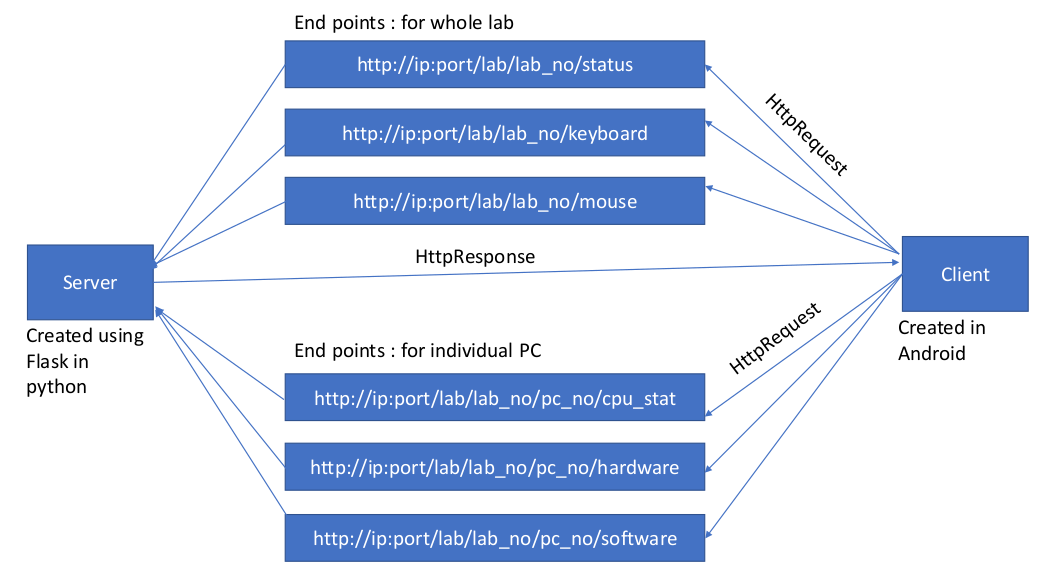
\includegraphics[scale=0.5]{assets/design.png}
        \caption{Design of System}
\end{figure}
\subsubsection{Server}
Server is implemented using Python and Flask server. The server will be in one of the lab system so that it can access all the systems present in the lab. Server will accept the requests made by remote client then it will perform all the necessary actions and then it will reply the client.
\subsubsection{Client}
Client is a android application implemented using Java and android studio. Client will take commands from the user and then it will send it to server and wait for server reply. Then it will give the output to the user.
\newpage

\subsection{Experimental Results}
\begin{figure}[H]
    \centering
        \begin{minipage}{0.46\textwidth}
            \centering
            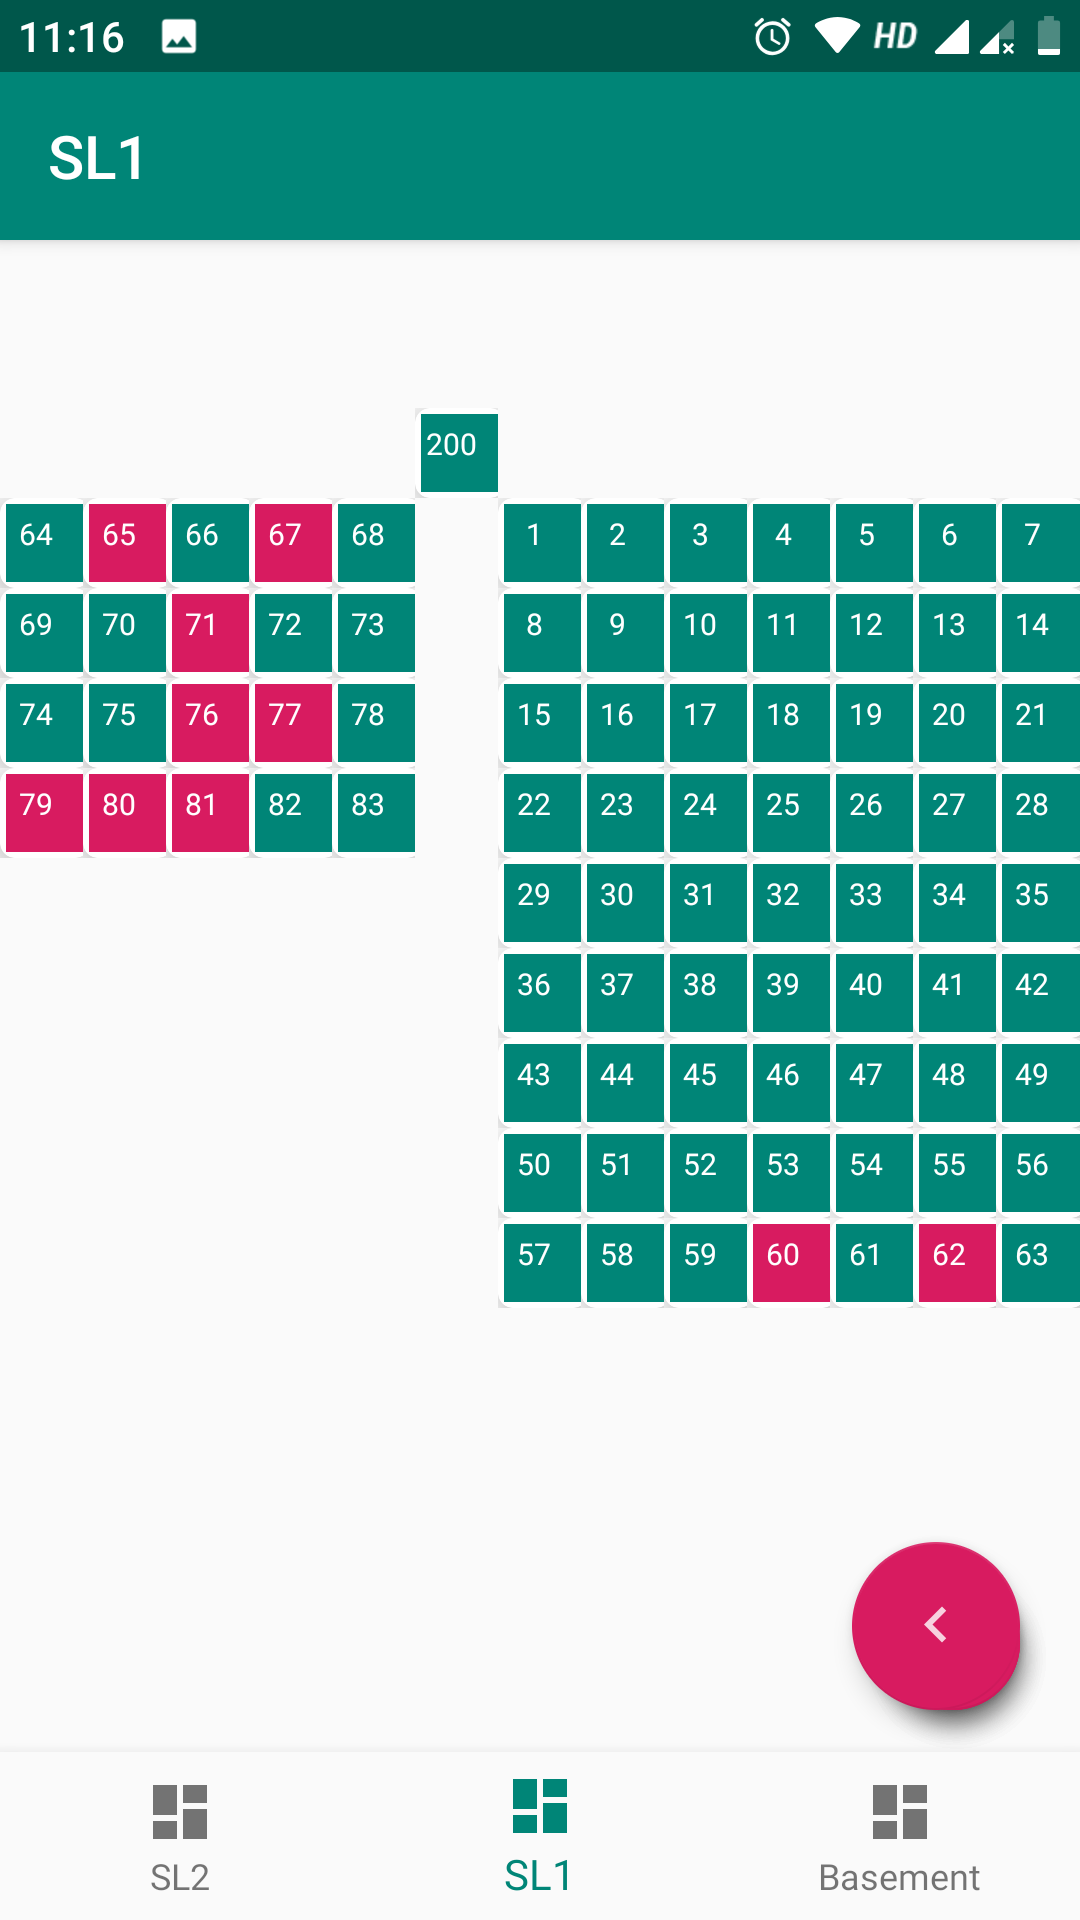
\includegraphics[width=5cm,height=8cm]{assets/SL1.png}
            \caption{Screenshot: Software Lab 1 status.}
        \end{minipage}\hfill
        \begin{minipage}{0.46\textwidth}
            \centering
            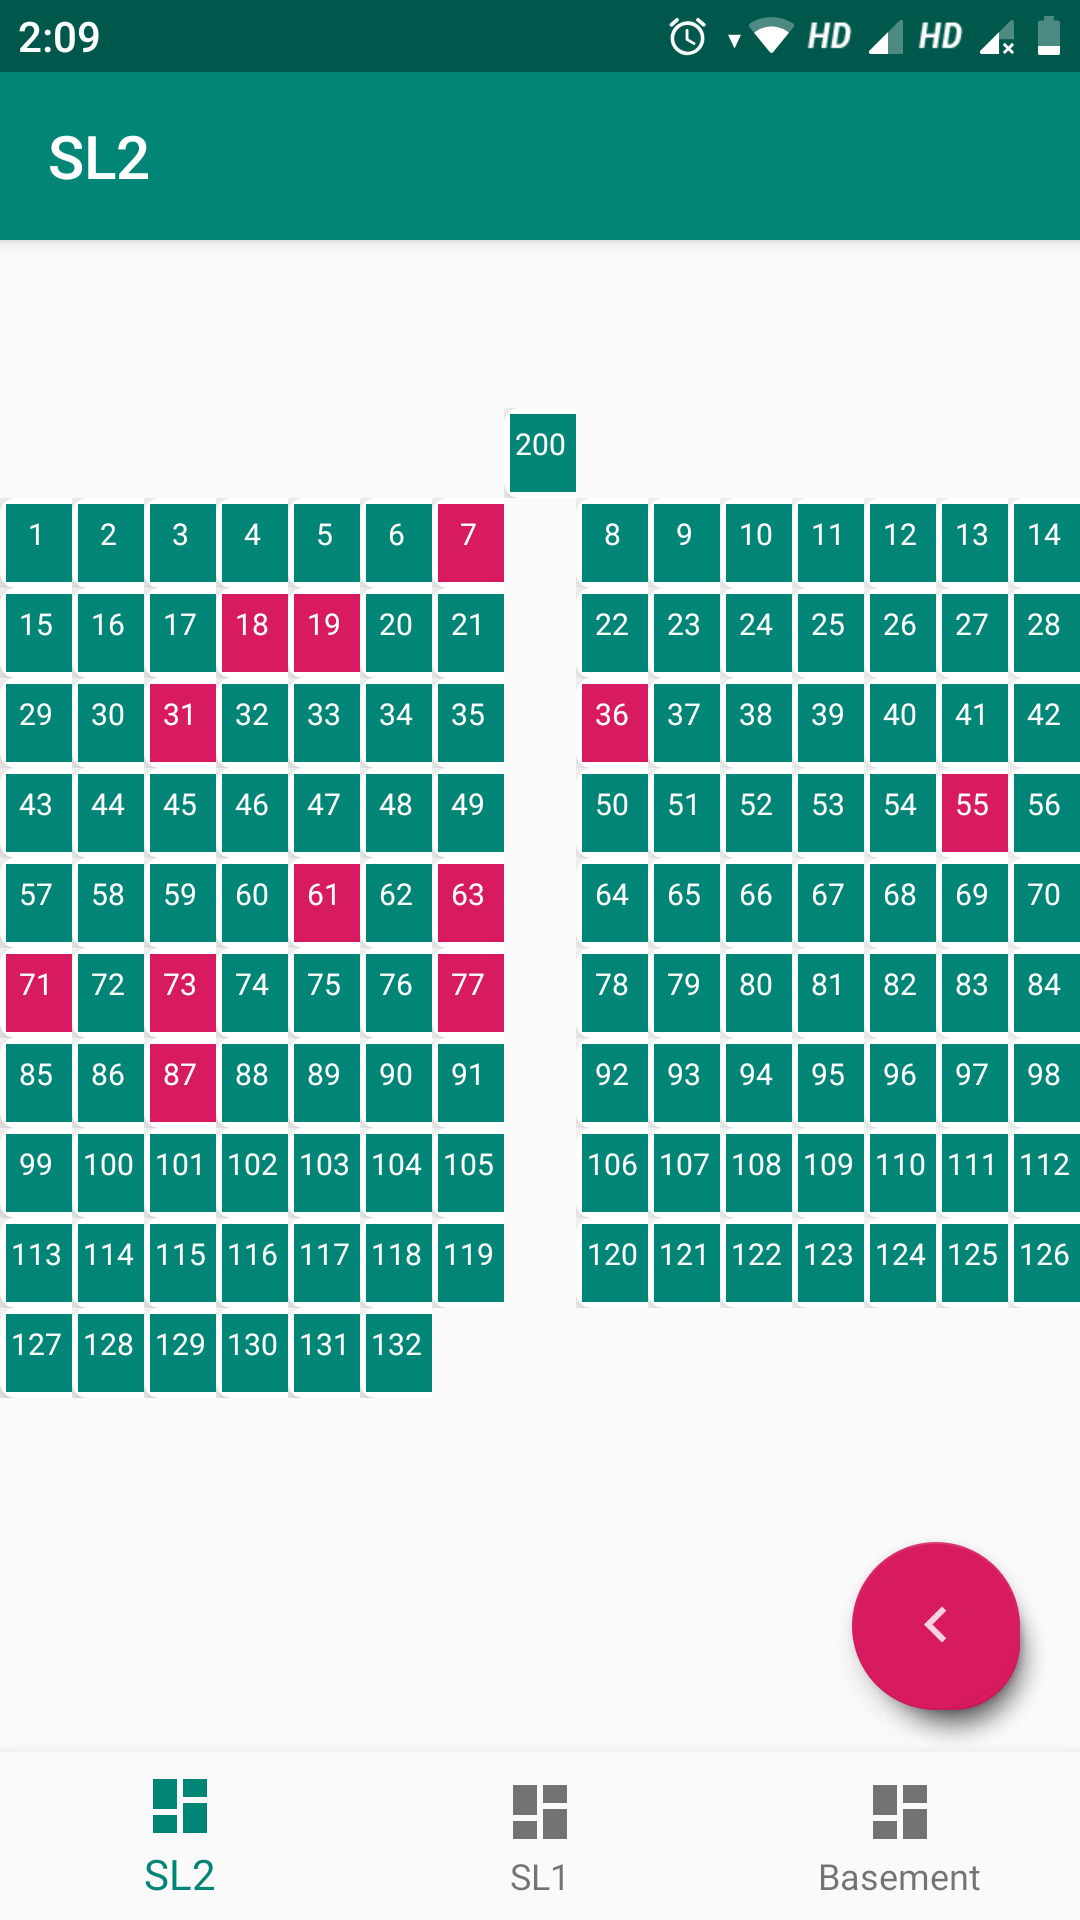
\includegraphics[width=5cm,height=8cm]{assets/SL2.png}
            \caption{Screenshot: Software Lab 2 status.}
        \end{minipage}\hfill
        \begin{minipage}{0.46\textwidth}
            \centering
            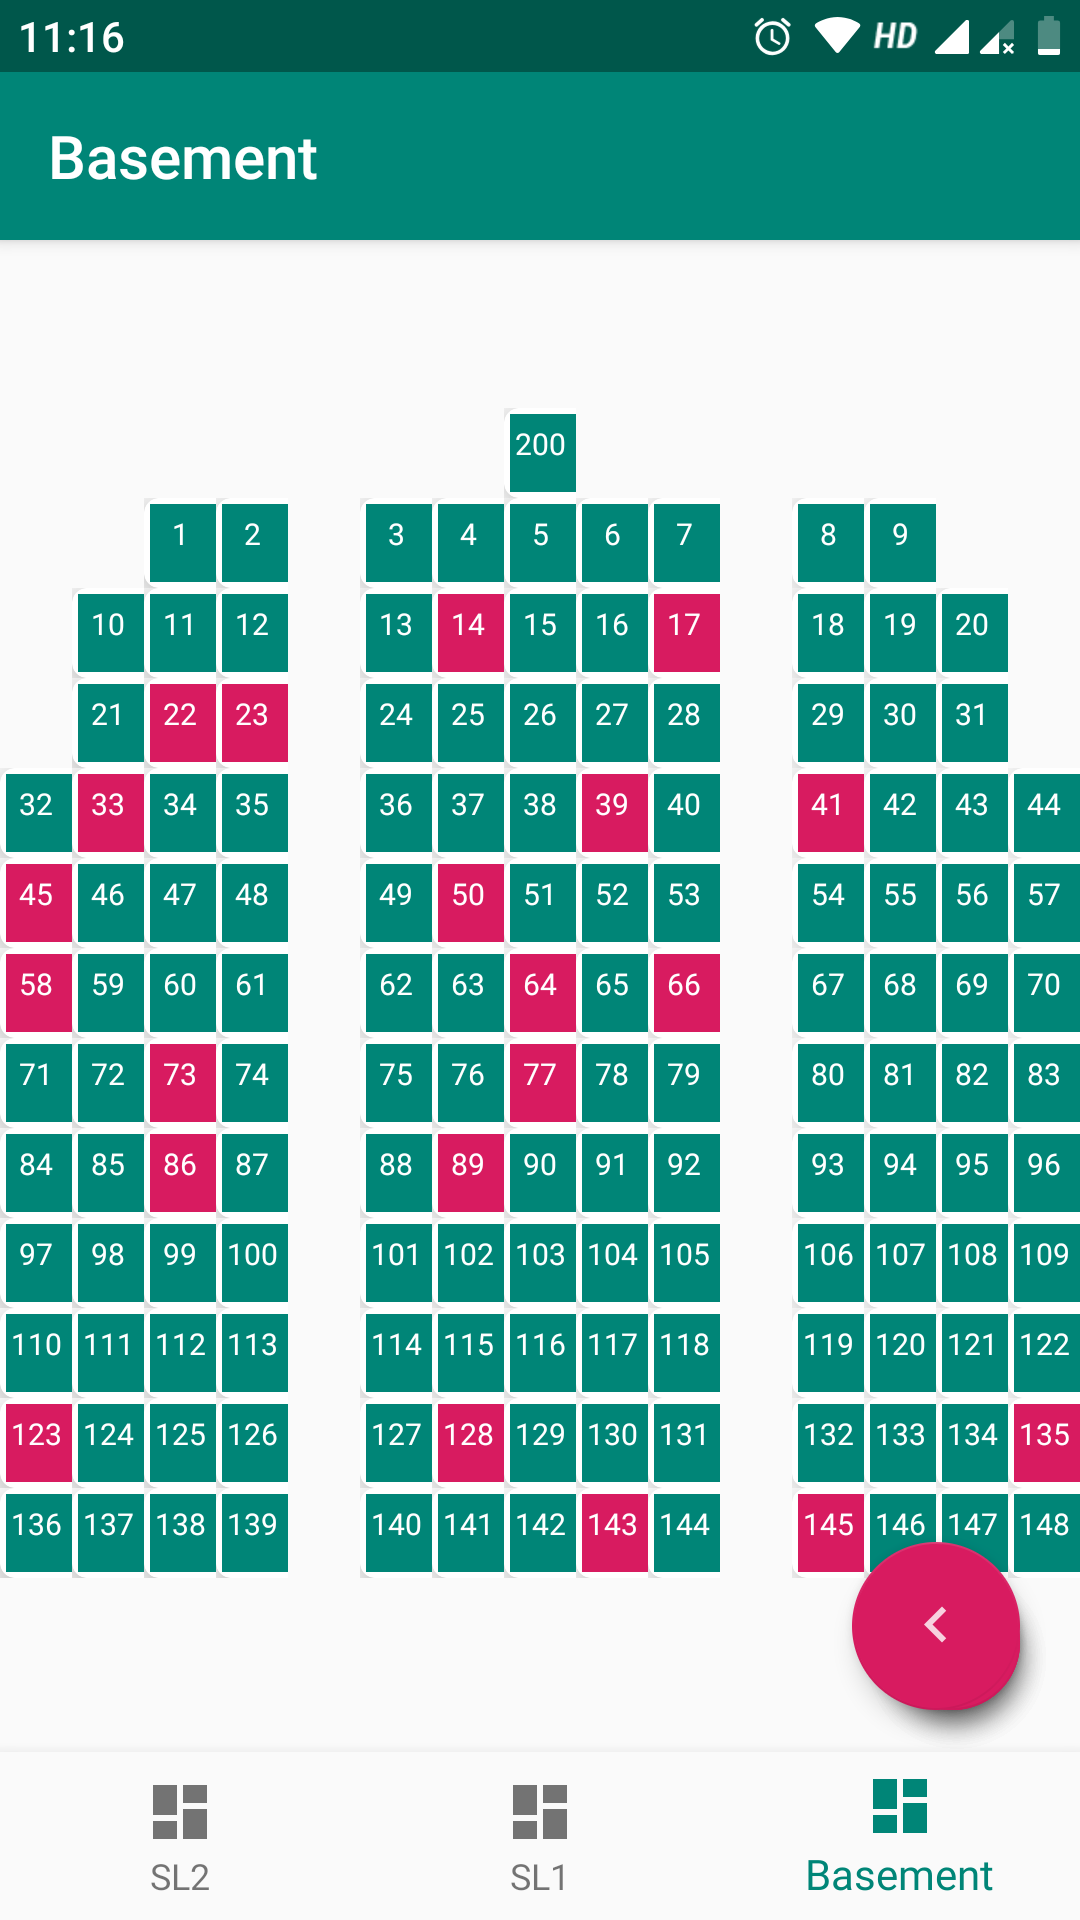
\includegraphics[width=5cm,height=8cm]{assets/Basement.png}
            \caption{Screenshot: Basement Lab status.}
        \end{minipage}\hfill
        \begin{minipage}{0.46\textwidth}
            \centering
            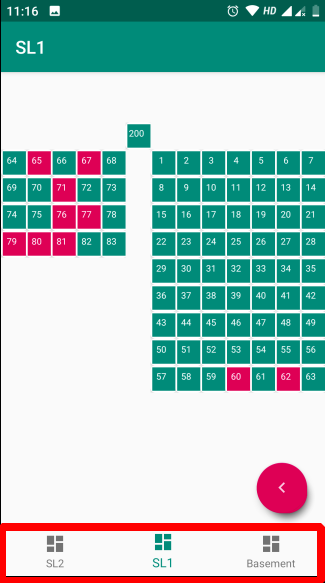
\includegraphics[width=5cm,height=8cm]{assets/slidebar.png}
            \caption{Screenshot: List of Labs.}
        \end{minipage}\hfill
\end{figure}
The above set of images shows the results of the android client. This shows lab status of various labs.
\begin{figure}[H]
    \centering
        \begin{minipage}{0.46\textwidth}
            \centering
            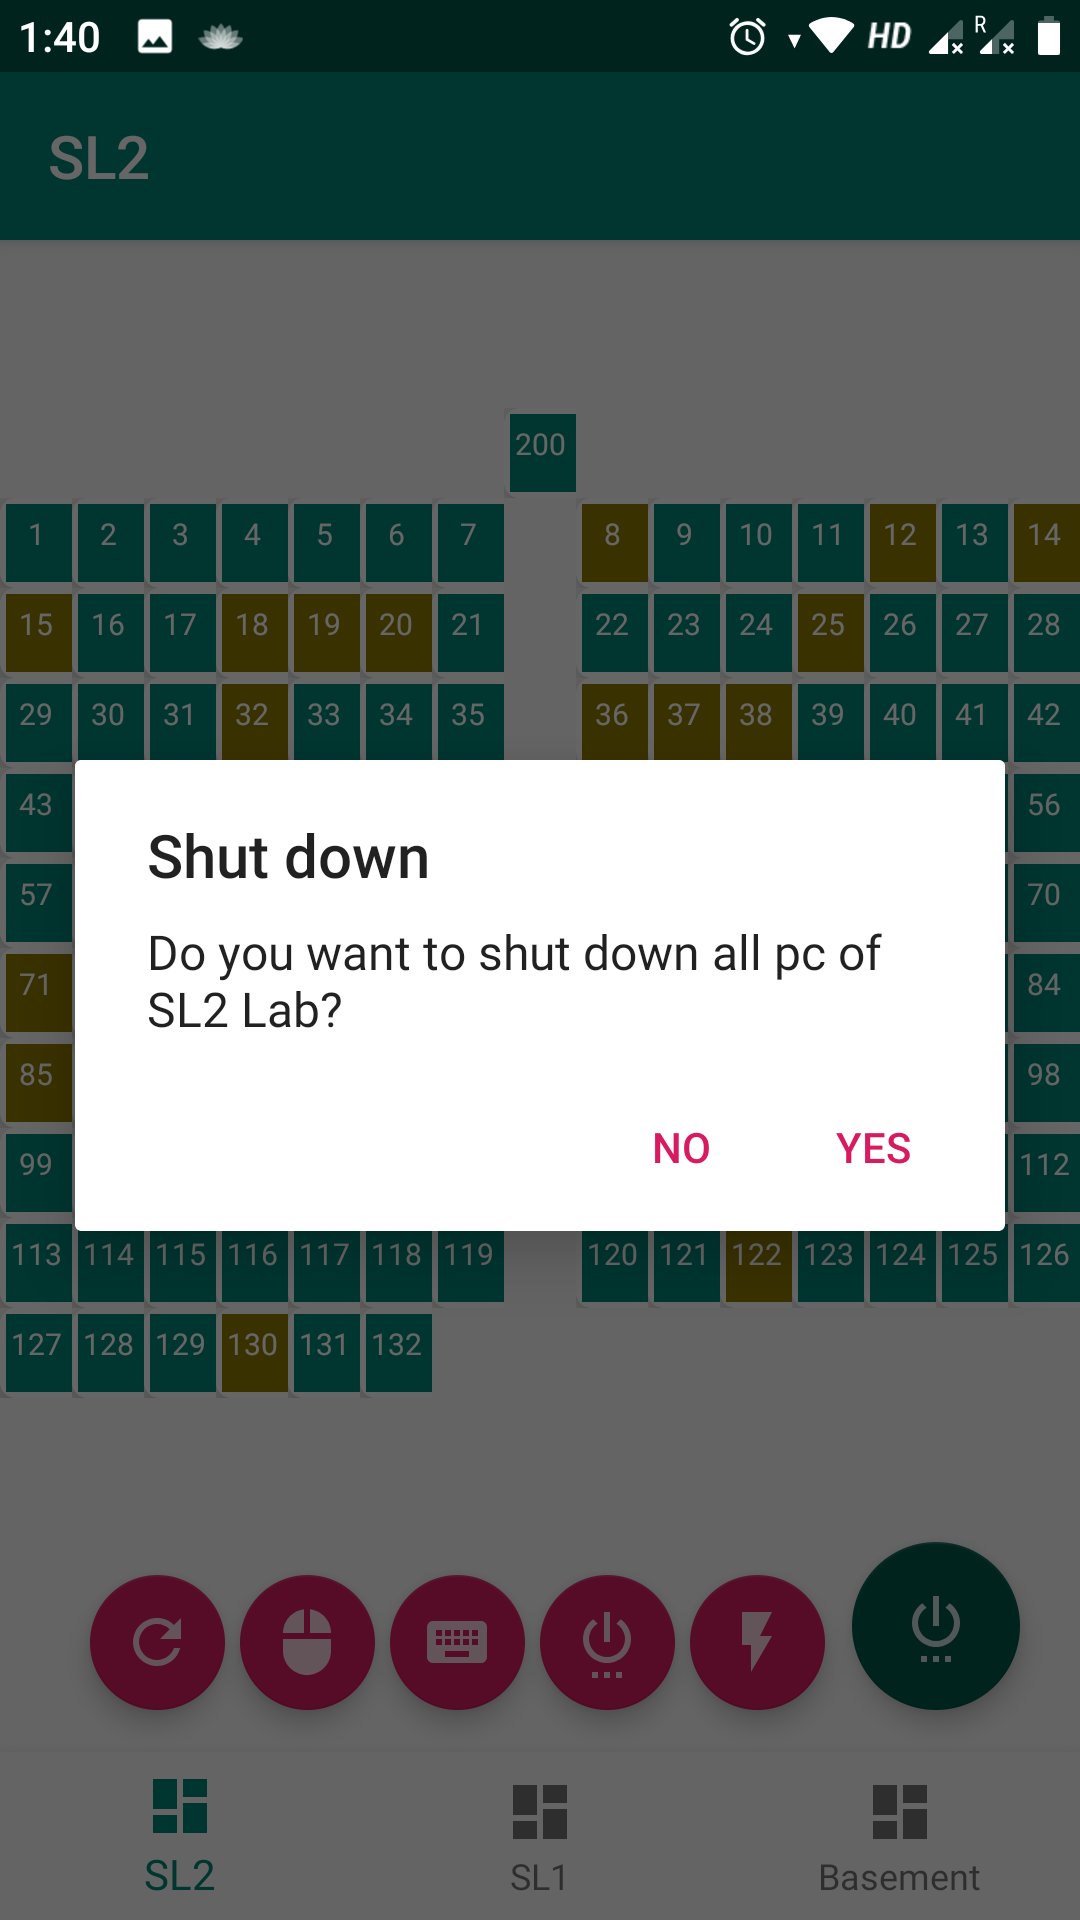
\includegraphics[width=5cm,height=8cm]{assets/ShutDownConfirm.png}
            \caption{Screenshot: Shut Down function.}
        \end{minipage}\hfill
        \begin{minipage}{0.46\textwidth}
            \centering
            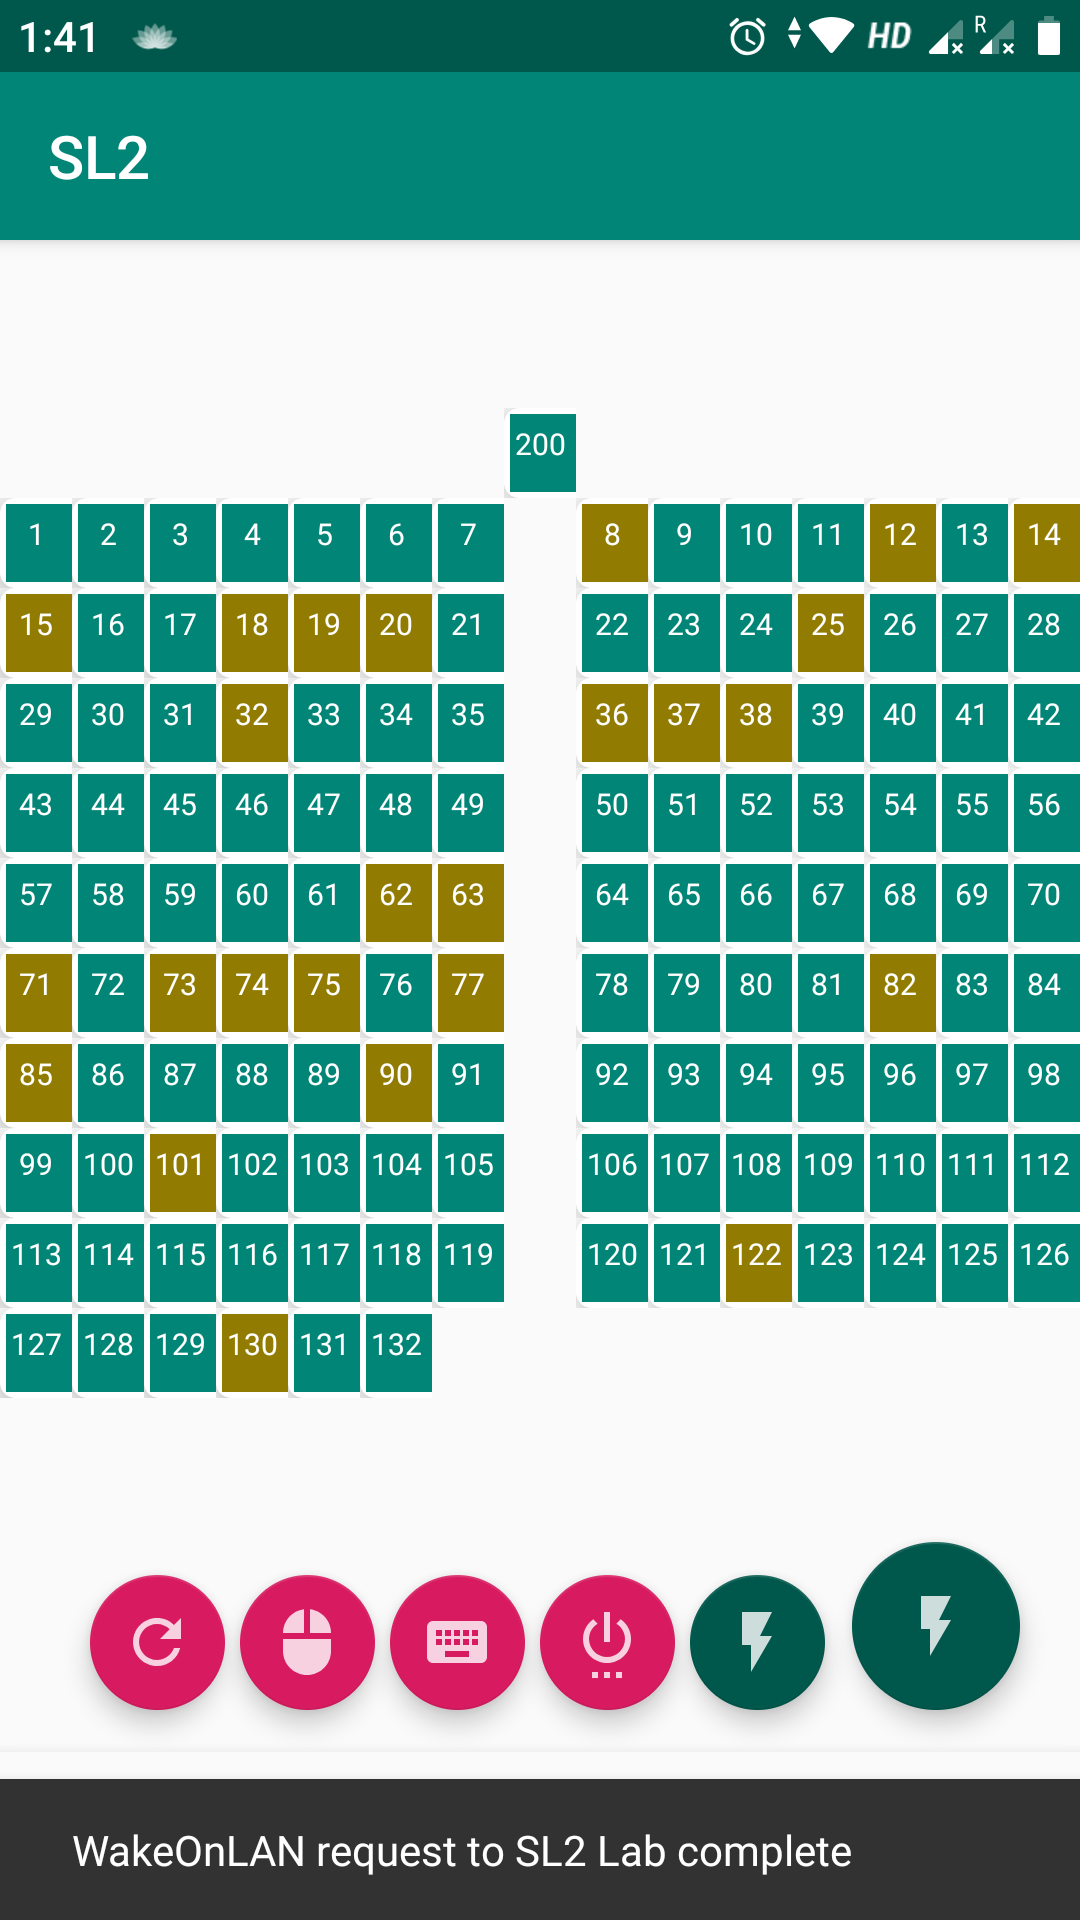
\includegraphics[width=5cm,height=8cm]{assets/WakeOnLan.png}
            \caption{Screenshot: Wake on lan function.}
        \end{minipage}\hfill
        \begin{minipage}{0.46\textwidth}
            \centering
            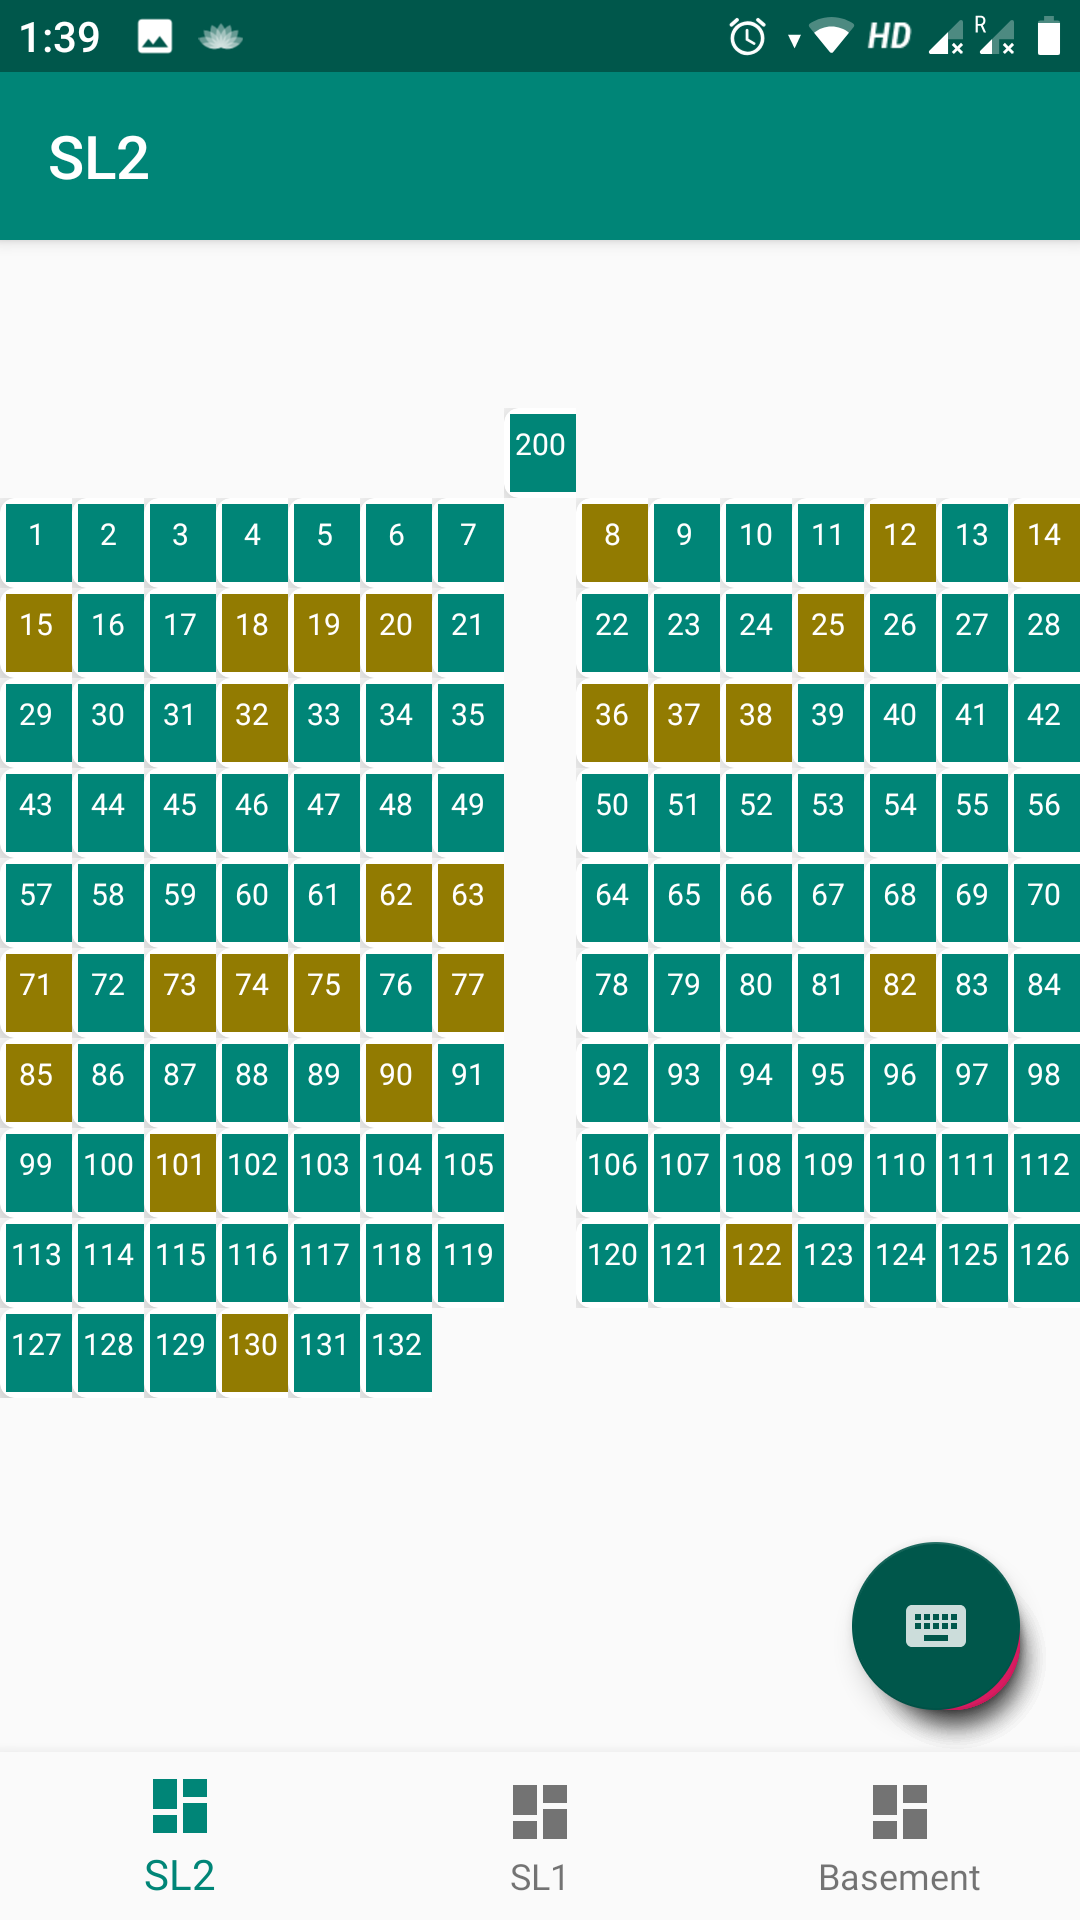
\includegraphics[width=5cm,height=8cm]{assets/Keybord.png}
            \caption{Screenshot: Keybord function.}
        \end{minipage}\hfill
        \begin{minipage}{0.46\textwidth}
            \centering
            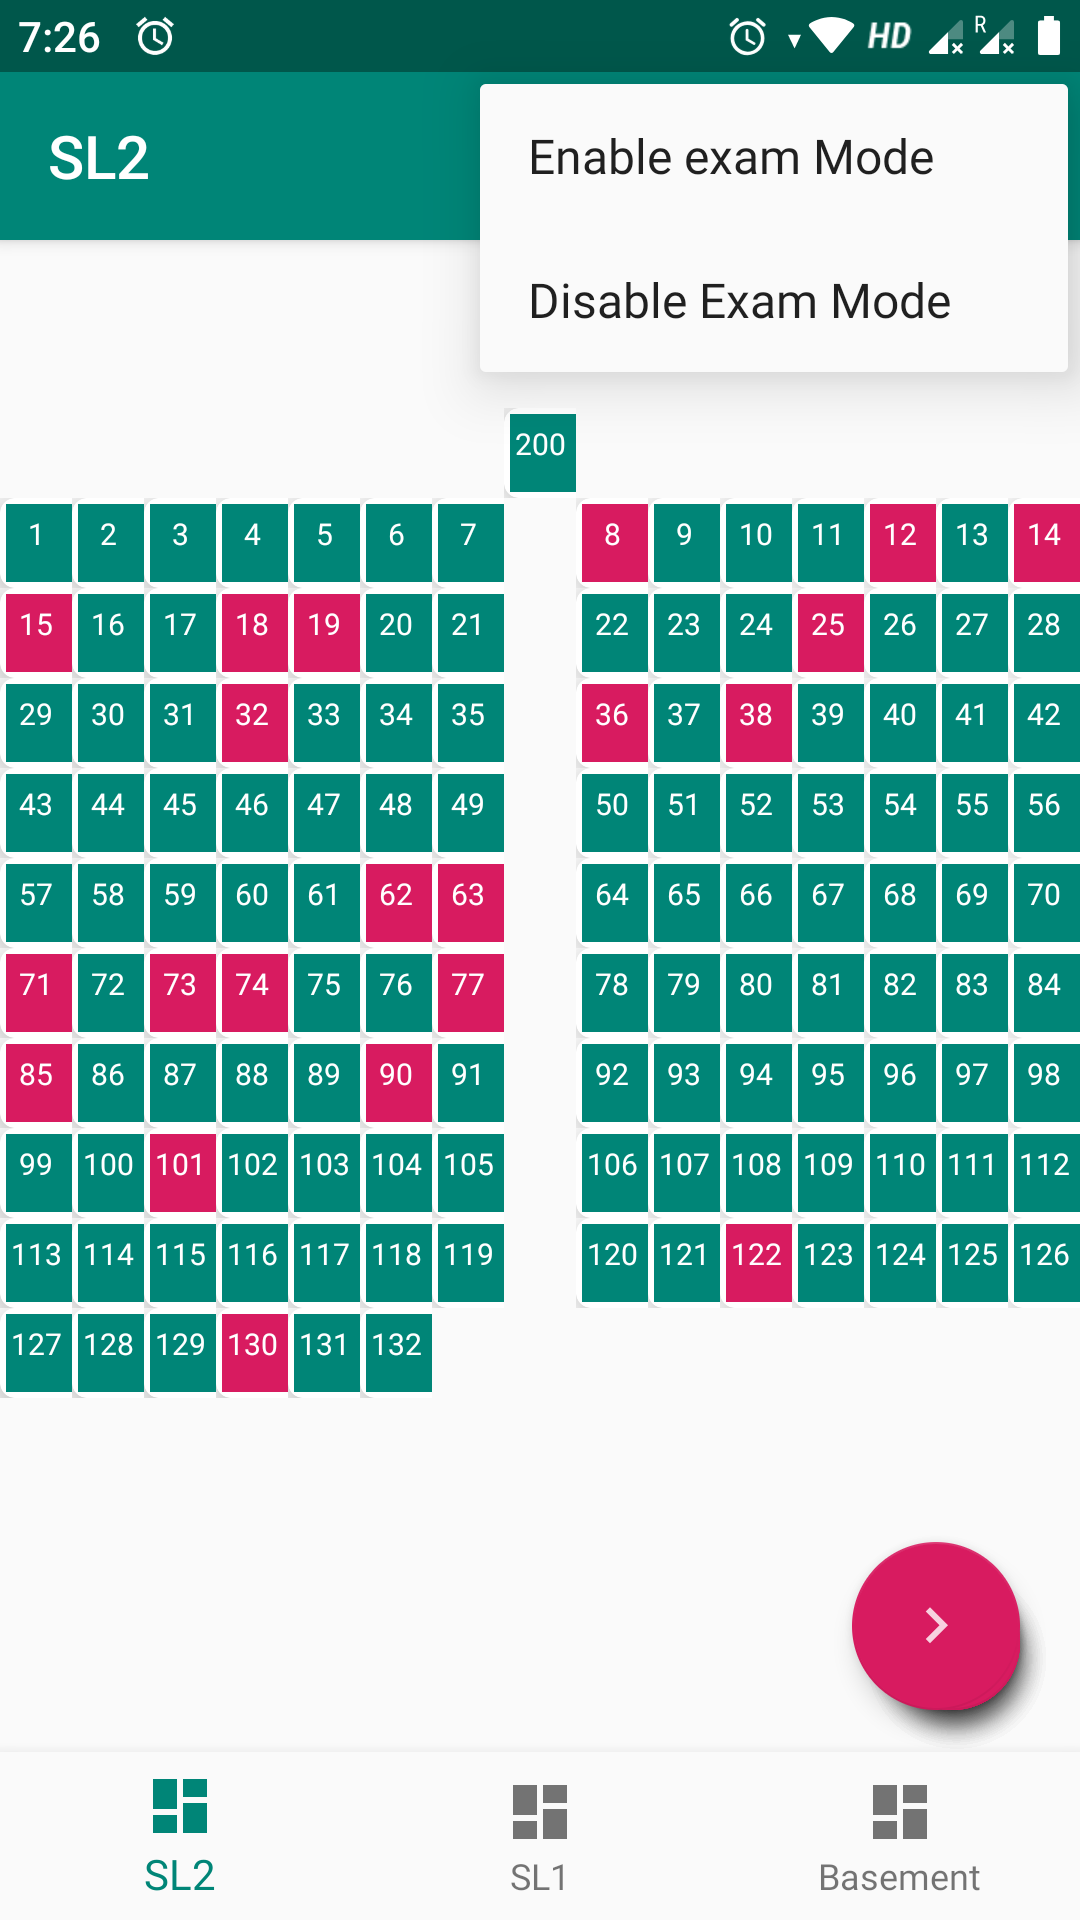
\includegraphics[width=5cm,height=8cm]{assets/exammode.png}
            \caption{Screenshot: Exam Mode option.}
        \end{minipage}\hfill       
\end{figure}
\subsection{Use Cases}
The following image shows the use case description of the android client. This diagram gives detailed description of monitoring individual system in particular lab.
\begin{figure}[H]
        \centering
        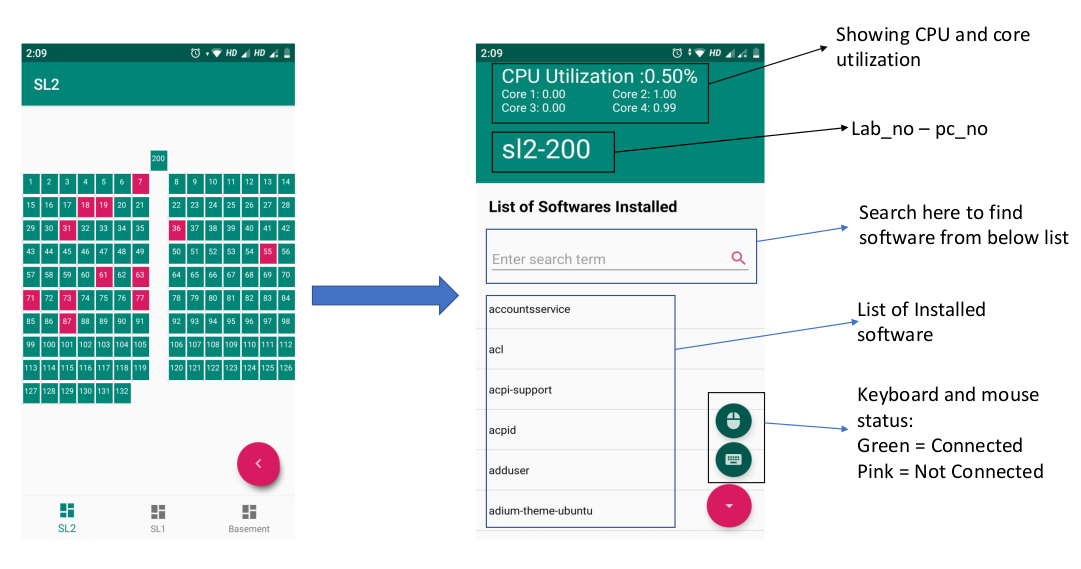
\includegraphics[scale=0.5]{assets/use_cases.png}
        \caption{Use Cases for client.}
\end{figure}
The following use case diagram shows the functionalities provided by the Lab Monitor. These are listed at bottom of the page. All the functionalities can be performed simultaniously on the one lab at a time and not multiple labs at same time.
\begin{figure}[H]
        \centering
        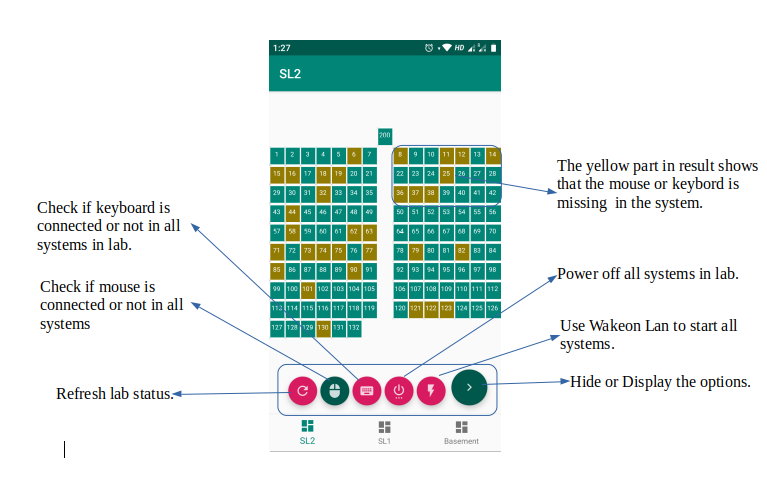
\includegraphics[scale=0.5]{assets/functionality.png}
        \caption{Use Cases for functionalities provided.}
\end{figure}

\newpage

\section{User Documentation}
The source code for this project is available on \href{https://github.com/prantostic/CS699}{GitHub} \\
Clone this to your system using following command.
\begin{verbatim} 
    git clone https://github.com/prantostic/CS699.git
    \end{verbatim}
\subsection{Server}
\begin{enumerate}

\item For running the server following are the requirements. Install them first%% {lstlisting}[language=sh] in place of verbatim 
    \begin{enumerate}
        \item python
        \begin{verbatim} 
            sudo apt-get update 
            sudo apt-get install python3.6
        \end{verbatim}
        \item pip3
        \begin{verbatim} 
            sudo apt install python3-pip
        \end{verbatim}
        \item paramiko==2.6.0
        \begin{verbatim}
            pip3 install paramiko
        \end{verbatim}
        \item pynacl==1.3.0
        \begin{verbatim}
            pip3 install pynacl
        \end{verbatim}
        \item flask==1.1.1
        \begin{verbatim}
            pip3 install flask
        \end{verbatim}
    \end{enumerate}

\item To run server go to the directory containing the project CS699. Open terminal in that directory. Go to the folder containing server code.
    \begin{verbatim}
        cd CS699/source/server
    \end{verbatim}

\item Main program for the project is app.py. Run this program for starting the server.
    \begin{verbatim}
    python3 app.py
    \end{verbatim}

\item After the server is up it will ask for the system administrator credentials.
Enter username and password.
Then the server will be on and it will start listening to client.
\end{enumerate}

\subsection{client}
\begin{enumerate}
    \item Android application(.apk) file is provided in git directory. You can directly install it in your android device.
    \item If you want to compile code in your system follow the steps below.
    \begin{enumerate}
        \item Following are the requirements for compiling client.
        \begin{enumerate}
            \item Java
            \item Android Studio
        \end{enumerate}
        \item You have to import the client code in Android Studio
        \begin{enumerate}
            \item Open android studio.
            \item Go to File\textrightarrow New\textrightarrow Import Project
            \item Choose the folder CS699/source/client/LabStatus
            \item Click Next\textrightarrow Finish
        \end{enumerate}
        \item Android Studio will build the project for you.
        \item You can now run the client project in Android Studio.
    \end{enumerate}
\end{enumerate}
\newpage

\section{Future Usage}
The Lab Monitor project is very useful in future as the further batches of system administrators will make use of it and it will be continued.
Lab Monitor will help system administrators in reducing the physical efforts.\\\\
Everything in our project is working in very good way but we will look forward to add more functionalities.


\newpage
\section{Conclusion}
We have built the client server model using which the system administrator will be able to perform their task effectively and fast. This app can provide details like is system connected to network, list of softwares installed, list of connected hardware devices, etc. User will also be able to shut down the systems as well as start the system remotely.
\newpage
\end{document}
